% !TEX options=--shell-escape
\documentclass[12pt]{article}
\usepackage{graphicx}
\usepackage{geometry}
\usepackage{amsmath}
\usepackage{float}
\usepackage{minted}
\geometry{margin=1.7cm}
\usepackage{xcolor}
\definecolor{LightGray}{gray}{0.9}
\usepackage{mathtools}
\DeclarePairedDelimiter{\ceil}{\lceil}{\rceil}
\usepackage{tikz}
\usetikzlibrary{automata, positioning, arrows}
% \tikzset{
%         ->,  % makes the edges directed
%         >=stealth, % makes the arrow heads bold
%         node distance=3cm, % specifies the minimum distance between two nodes. Change if nevery state/.
%         style={thick, fill=gray!10}, % sets the properties for each ’state’ n
%         initial text=$ $, % sets the text that appears on the start arrow
%         }
% \definecolor{lgrey}{gray}{.96}

%
% Title.
\title{Experiment 3: String recogniser}
% Author
\author{\textit{Parthasarathi Khirwadkar}\\\textit{16D070001}}

% begin the document.
\begin{document}

% make a title page.
\maketitle

% section 1: overview.
\section*{Overview}
In this experiment, I have used sequential circuits and the concept of Mealy FSM to implement a string recognizer. The function of this circuit is to recognize the occurrence of specific strings hidden in plain text.\\
The input to the circuit is in the form of sequence of 5 bit vectors which encode the alphabet, 1 bit for reset and a clock signal which in this case was provided using 1 bit. Thus the circuit takes 7 bits of input at once. The circuit is able to recognize the following strings:
% % In two to three paragraphs, summarize 
\begin{itemize}
\item Gun
\item Bomb
\item Knife
\item Terror
\end{itemize}

The code was compiled on \textbf{Quartus Prime} and tested using \textbf{ModelSim} for RTL and Gate-level simulations. The code was then uploaded to \textbf{Krypton v1.1 5M1270ZT144C5N} CPLD-based board. The circuit was then tested using scan chain.

% You may refer to pre-existing documents by
% citing them appropriately \cite{ref:Ramayana}.

% For a more detailed introduction to the use of
% LaTex to write documents, see \cite{ref:LatexTutorial}.

% section 2: setup/approach.
\section{Setup}
The input character set which is the English alphabet consists of 26 characters. To encode these a minimum of $\ceil{log_2 26} = 5$ bits are required. For simplicity, I used the binary encoding ,where a = 1, for this purpose as it uses minimum number of bits. A reset bit and a clock bit was also added for reseting the string recognizer for testing purpose and to control the circuit.\\
The string recognizer circuit consists of individual FSMs connected in parallel which detect the occurrence of one particular string. The outputs of these individual FSMs are passed through an OR gate to get the required output.\\

\subsection{``Gun" Recogniser}
The state transition diagram for the FSM which recognizes ``gun'' is as follows:
\begin{figure}[H] % ’ht’ tells LaTeX to place the figure ’here’ or at the top of the page
    \centering % centers the figure
    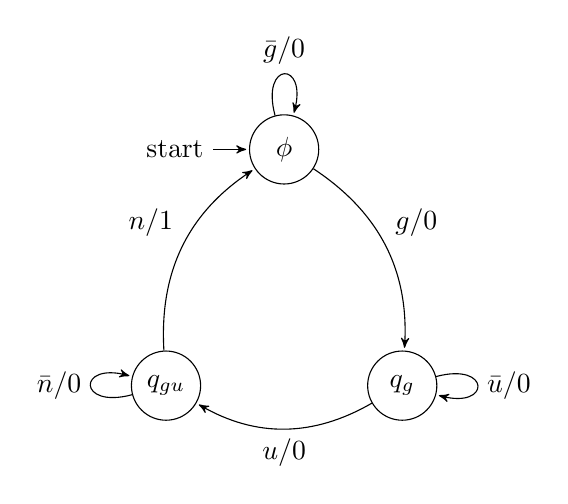
\begin{tikzpicture}[>=stealth',shorten >=1pt,auto,node distance=2cm]
        % tikz code goes here
        \node[state,initial](phi) at (1.5,3) {$\phi$};
        \node[state](q_g) at (3,0){$q_g$};
        \node[state](q_gu) at (0,0){$q_{gu}$};
        % \draw[->] (phi) edge[loop above] {\tt 0} (phi);
        \path[->]	(phi)	edge [loop above]	node {$\bar{g}/0$}	(phi)
        		  			edge [bend left] 	node {$g/0$} 		(q_g)
        			(q_g)	edge [bend left]	node {$u/0$}		(q_gu)
        					edge [loop right]	node {$\bar{u}/0$}	(q_g)
        			(q_gu)	edge [bend left]	node {$n/1$}		(phi)
        					edge [loop left]	node {$\bar{n}/0$}	(q_gu);

    \end{tikzpicture}
    \caption{State Diagram of ``gun'' recognizer}
    % \label{fig:my_label}
\end{figure}
The edge labels of the state machine is in the format input/output.
To encode the state, I have used binary encoding in this case.
\begin{table}[H]
	\centering
	\begin{tabular}{|c|c|c|}
	\hline
	\textbf{State} 	& $q_1$	& $q_0$ \\
	\hline
	$\phi$	& 0 	& 0		\\
	$q_g$	& 0 	& 1		\\
	$q_{gu}$& 1 	& 0		\\
	\hline
	\end{tabular}
	\caption{Encoding of states of ``gun'' recognizer}
\end{table}
% \inputminted[bgcolor=LightGray]{vhdl}{vhdl_files/xor2.vhd}  

Next, the implementation of ``gun'' recognizer is as follows:

\inputminted[bgcolor=LightGray]{vhdl}{code/gun_recog.vhd}

\subsection{``Bomb" Recogniser}
The state transition diagram for the FSM which recognizes ``bomb'' is as follows:
\begin{figure}[H] % ’ht’ tells LaTeX to place the figure ’here’ or at the top of the page
    \centering % centers the figure
    \begin{tikzpicture}[>=stealth',shorten >=1pt,auto,node distance=2cm]
        % tikz code goes here
        \node[state,initial](phi) at (2.5,3) {$\phi$};
        \node[state](q_b) at (5,0){$q_b$};
        \node[state](q_bo) at (2.5,-3){$q_{bo}$};
        \node[state](q_bom) at (0,0){$q_{bom}$};
        % \draw[->] (phi) edge[loop above] {\tt 0} (phi);
        \path[->]	(phi)	edge [loop above]	node {$\bar{b}/0$}	(phi)
        		  			edge [bend left] 	node {$b/0$} 		(q_b)
        			(q_b)	edge [bend left]	node {$o/0$}		(q_bo)
        					edge [loop right]	node {$\bar{o}/0$}	(q_b)
        			(q_bo)	edge [bend left]	node {$m/0$}		(q_bom)
        					edge [loop below]	node {$\bar{m}/0$}	(q_bo)
        			(q_bom)	edge [bend left]	node {$b/1$}		(phi)
        					edge [loop left]	node {$\bar{b}/0$}	(q_bom);

    \end{tikzpicture}
    \caption{State Diagram of ``bomb'' recognizer}
    % \label{fig:my_label}
\end{figure}
The edge labels of the state machine is in the format input/output.
To encode the state, I have used binary encoding in this case.
\begin{table}[H]
	\centering
	\begin{tabular}{|c|c|c|}
	\hline
	\textbf{State} 	& $q_1$	& $q_0$ \\
	\hline
	$\phi$	& 0 	& 0		\\
	$q_b$	& 0 	& 1		\\
	$q_{bo}$& 1 	& 0		\\
	$q_{bom}$& 1 	& 1		\\
	\hline
	\end{tabular}
	\caption{Encoding of states of ``bomb'' recognizer}
\end{table}
% \inputminted[bgcolor=LightGray]{vhdl}{vhdl_files/xor2.vhd}  

The implementation of ``bomb'' recognizer is as follows:

\inputminted[bgcolor=LightGray]{vhdl}{code/bomb_recog.vhd}

\subsection{``Knife" Recogniser}
The state transition diagram for the FSM which recognizes ``knife'' is as follows:
\begin{figure}[H] % ’ht’ tells LaTeX to place the figure ’here’ or at the top of the page
    \centering % centers the figure
    \begin{tikzpicture}[>=stealth',shorten >=1pt,auto,node distance=2cm]
        % tikz code goes here
        \node[state,initial](phi) at (1.5,6) {$\phi$};
        \node[state](q_k) at (4.5,3){$q_k$};
        \node[state](q_kn) at (3,0){$q_{kn}$};
        \node[state](q_kni) at (0,0){$q_{kni}$};
        \node[state](q_knif) at (-1.5,3){$q_{knif}$};
        % \draw[->] (phi) edge[loop above] {\tt 0} (phi);
        \path[->](phi)	edge [loop above]	node {$\bar{k}/0$}	(phi)
        				edge [bend left] 	node {$k/0$} 		(q_k)
        		(q_k)	edge [bend left]	node {$n/0$}		(q_kn)
        				edge [loop right]	node {$\bar{n}/0$}	(q_k)
        		(q_kn)	edge [bend left]	node {$i/0$}		(q_kni)
        				edge [loop below]	node {$\bar{i}/0$}	(q_kn)
        		(q_kni)	edge [loop below]	node {$\bar{f}/0$}	(q_kni)
        				edge [bend left]	node {$f/0$}		(q_knif)
        		(q_knif)edge [bend left]	node {$e/1$}		(phi)
        				edge [loop left]	node {$\bar{e}/0$}	(q_knif);


    \end{tikzpicture}
    \caption{State Diagram of ``knife'' recognizer}
    % \label{fig:my_label}
\end{figure}
The edge labels of the state machine is in the format input/output.
To encode the state, I have used gray codes encoding in this case. In this type of encoding, only single bit change occurs when going from one state to other. This also reduces error occurrence as we only have to ensure one bit change during each transition. It turns out that the combinational logic gets simplified much easily using this encoding and that is helpful in this case as the number of states is larger.
\begin{table}[H]
	\centering
	\begin{tabular}{|c|c|c|c|}
	\hline
	\textbf{State} 	& $q_2$	& $q_1$ & $q_0$ \\
	\hline
	$\phi$		& 0 & 0	& 0	\\
	$q_k$		& 0 & 0	& 1	\\
	$q_{kn}$	& 0 & 1	& 1	\\
	$q_{kni}$	& 0 & 1	& 0	\\
	$q_{knif}$	& 1 & 1	& 0	\\
	\hline
	\end{tabular}
	\caption{Encoding of states of ``knife'' recognizer}
\end{table}

The implementation of ``knife'' recognizer is as follows:

\inputminted[bgcolor=LightGray]{vhdl}{code/knife_recog.vhd}

\subsection{``Terror" Recogniser}
The state transition diagram for the FSM which recognizes ``terror'' is as follows:
\begin{figure}[H] % ’ht’ tells LaTeX to place the figure ’here’ or at the top of the page
    \centering % centers the figure
    \begin{tikzpicture}[>=stealth',shorten >=1pt,auto,node distance=2cm]
        % tikz code goes here
        \node[state,initial](phi) at (0,8) {$\phi$};
        \node[state](q_t) at (3,5){$q_t$};
        \node[state](q_te) at (3,2){$q_{te}$};
        \node[state](q_ter) at (0,0){$q_{ter}$};
        \node[state](q_terr) at (-3,2){$q_{terr}$};
        \node[state](q_terro) at (-3,5){$q_{terro}$};
        % \draw[->] (phi) edge[loop above] {\tt 0} (phi);
        \path[->](phi)	edge [loop above]	node {$\bar{t}/0$}	(phi)
        				edge [bend left] 	node {$t/0$} 		(q_t)
        		(q_t)	edge [bend left]	node {$e/0$}		(q_te)
        				edge [loop right]	node {$\bar{e}/0$}	(q_t)
        		(q_te)	edge [bend left]	node {$r/0$}		(q_ter)
        				edge [loop right]	node {$\bar{r}/0$}	(q_te)
        		(q_ter)	edge [loop below]	node {$\bar{r}/0$}	(q_ter)
        				edge [bend left]	node {$r/0$}		(q_terr)
        		(q_terr)edge [loop left]	node {$\bar{o}/0$}	(q_terr)
        				edge [bend left]	node {$o/0$}		(q_terro)	
        	(q_terro)	edge [loop left]	node {$\bar{r}/0$}	(q_terro)
        				edge [bend left]	node {$r/1$}		(phi);


    \end{tikzpicture}
    \caption{State Diagram of ``knife'' recognizer}
    % \label{fig:my_label}
\end{figure}
The edge labels of the state machine is in the format input/output.
To encode the state, similar to ``knife'' recognizer, I have used gray codes encoding in this case. 
\begin{table}[H]
	\centering
	\begin{tabular}{|c|c|c|c|}
	\hline
	\textbf{State} 	& $q_2$	& $q_1$ & $q_0$ \\
	\hline
	$\phi$		& 0 & 0	& 0	\\
	$q_t$		& 0 & 0	& 1	\\
	$q_{te}$	& 0 & 1	& 1	\\
	$q_{ter}$	& 0 & 1	& 0	\\
	$q_{terr}$	& 1 & 1	& 0	\\
	$q_{terro}$	& 1 & 1	& 1	\\
	\hline
	\end{tabular}
	\caption{Encoding of states of ``terror'' recognizer}
\end{table}

The implementation of ``terror'' recognizer is as follows:

\inputminted[bgcolor=LightGray]{vhdl}{code/terror_recog.vhd}

\subsection{Putting everything together - String Recognizer} % (fold)
\label{sub:putting_everything_together_string_recognizer}
Now that we have got the 4 individual FSMs working, we can build the string recognizer by simply connecting the 4 FSM in parallel and putting the output of all FSMs through a 4-bit OR gate. All the 4 FSM are provided the same clock and reset signal. Here's the implementation:

\inputminted[bgcolor=LightGray]{vhdl}{code/string_recog.vhd}
% subsection putting_everything_together_string_recognizer (end)

\subsection{Testbench} % (fold)
\label{sub:testbench}
Following is the testbench used for this experiment:
\inputminted[bgcolor=LightGray]{vhdl}{code/testbench.vhd}
% subsection testbench (end)

\section{Observations}

The circuit was simulated using ModelSim for RTL and Gate level simulation. Next, the code was uploaded onto the Krypton board and using scan chain, the circuit was tested. Following are the results of RTL, Gate level simulation and scan chain testing of the string recogniser.

\begin{figure}[H]
	\centering
	\includegraphics[width=0.9\textwidth]{rtl_sim.png}
	\caption{RTL Simulation of String recognizer circuit}
\end{figure}

\begin{figure}[H]
	\centering
	\includegraphics[width=0.9\textwidth]{gate_lvl.png}
	\caption{Gate Level Simulation of String recognizer circuit}
\end{figure}

\begin{figure}[H]
	\centering
	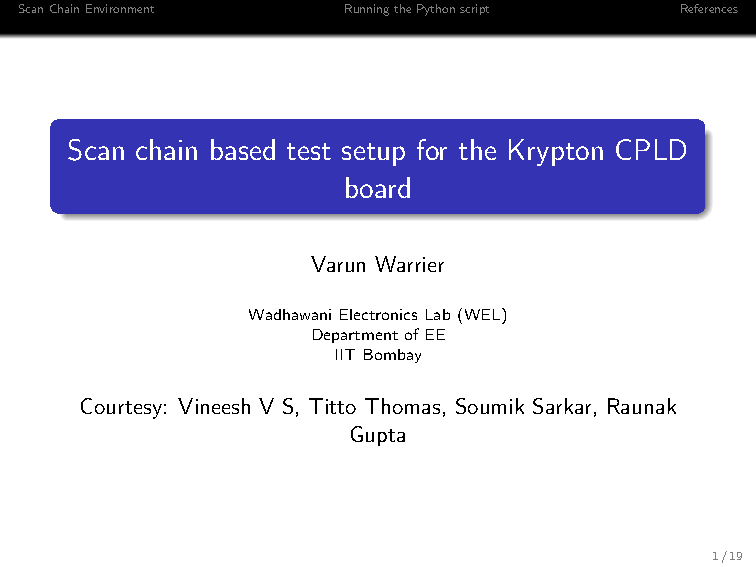
\includegraphics[width=0.9\textwidth]{scan_chain.png}
	\caption{Scan Chain Result of String recognizer circuit}
\end{figure}

\end{document}
